\documentclass{article}

\usepackage[final]{neurips_2019}

\usepackage[utf8]{inputenc}
\usepackage[T1]{fontenc}
\usepackage{hyperref}
\usepackage{url}
\usepackage{booktabs}
\usepackage{amsfonts}
\usepackage{nicefrac}
\usepackage{microtype}
\usepackage{graphicx}
\usepackage{xcolor}
\usepackage{lipsum}

\newcommand{\note}[1]{\textcolor{blue}{{#1}}}

\title{
  GAN Enabled Drone Trajectory Prediction \\
  \vspace{1em}
  \small{\normalfont Stanford CS236G Final Project} 
}

\author{
  Akram Sbaih \\
  Department of Computer Science \\
  Stanford University \\
  \texttt{akram@stanford.edu} \\
     \And
   \texttt{Mentor} Eric Zelikman \\
   Department of Computer Science \\
   Stanford University \\
   \texttt{ezelikman@cs.stanford.edu} \\
}

\begin{document}

\maketitle

% \begin{abstract}
%   Required for final report
% \end{abstract}


%\note{This template is built on NeurIPS 2019 template\footnote{\url{https://www.overleaf.com/latex/templates/neurips-2019/tprktwxmqmgk}} and provided for your convenience.}

\note{Code available at \href{https://github.com/aksbaih/drone-trajectory}{https://github.com/aksbaih/drone-trajectory}.}

\paragraph{Dataset.}$ $
\\\\ I'm using the UZH FPV Dataset \cite{Delmerico19icra} for this project. The authors of this dataset wanted to challenge the state of the art state estimation models in UAV racing by introducing highspeed manuevers in real-world environments. This task aims to approximate the trajectory and momentum of the drone based on minimal sensory input (in this case, the grayscale view through a camera attached to the drone). The dataset consists of frames taken at 50Hz tied to a ground truth representing the momentum around each of the 6 degrees of freedom the drone has in 16 flights lasting around 100 seconds each. 
\\\\ I'm reusing the dataset for a different task here: I'm interested in predicting the immediate trajectory of a drone based on its location history as observed from a third-party. This trajectory info is embedded in the ground truth of the original dataset. Therefore, I use the dataset toolbox and my own code in the linked repo to generate the xyz location of the drone at each frame of a constant FPS and store it locally as a txt file for each flight.  Since I'm going to be using transformers, I reduce the FPS to 8 instead of 50 to span larger trajectory in less memory but this is subject to change based on later experiments.  This totals 11486 frames.  Figure \ref{DatasetExamples} shows example trajectories.
\\\\ Since the number of flights is not very big and each flight has a different pattern of trajectories, I reused the method of \cite{giuliari2020transformer} where the validation set is sampled as random windows of the training set when constructing the dataloader. 
I'm using 64 frames from each flight for validation, making around 9\% (1k frames) of all frames, but this could increase if needed. For the testing set, I left aside two flights that were considered "medium" according to \citep{Delmerico19icra} consisting of 1.9k frames, or 17\% of the original count. This leaves 74\% (8.6k frames) for training.
\begin{figure}
    \centering
    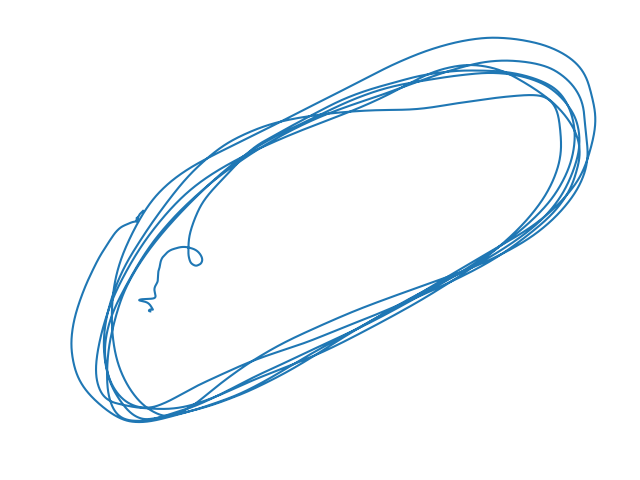
\includegraphics[width=0.35\textwidth]{indoor_forward_3.png}
    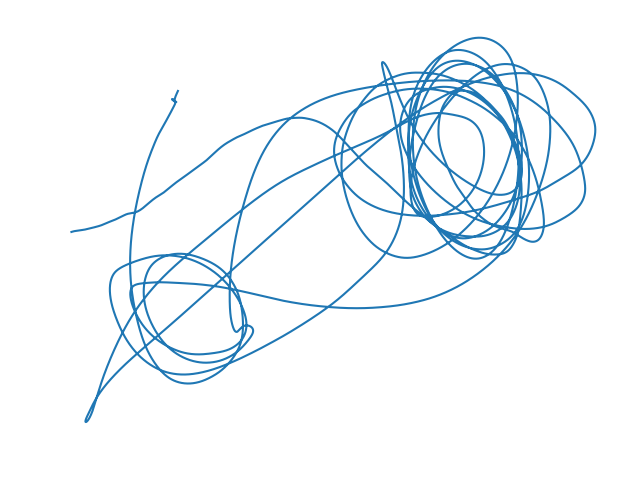
\includegraphics[width=0.35\textwidth]{indoor_forward_7.png}  \\
    \caption{Example flight trajectories from the UZH FPV Dataset \cite{Delmerico19icra}}
    \label{DatasetExamples}
\end{figure}

\bibliographystyle{unsrt}
\bibliography{references}

\end{document}
